\section{栈与队列}

\subsection{栈的定义与ADT}

\begin{mydef}{栈}{stack-def}
栈（Stack）是一种\textbf{操作受限}的线性表：只允许在表的一端进行插入和删除。这一端称为\textbf{栈顶}（Top），另一端称为\textbf{栈底}（Bottom）。

栈的操作遵循\textbf{后进先出}（LIFO, Last In First Out）原则：最后入栈的元素最先出栈。如同弹匣——后压入的子弹先弹出。

称插入操作为\textbf{入栈}（Push），称删除操作为\textbf{出栈}（Pop）。
\end{mydef}

\begin{conclusion}{栈的抽象数据类型（ADT）}{adt-stack}
栈 ADT 的核心操作集：
\begin{tablebox}{栈 ADT 操作}
\centering
\begin{tabular}{|c|l|}
\hline
操作 & 语义 \\
\hline
\texttt{InitStack(\&S)} & 初始化空栈 \\
\texttt{DestroyStack(\&S)} & 销毁栈，释放空间 \\
\texttt{StackEmpty(S)} & 判空，返回 bool \\
\texttt{StackLength(S)} & 返回栈中元素个数 \\
\texttt{GetTop(S, \&e)} & 取栈顶元素（不出栈）\\
\texttt{Push(\&S, e)} & 入栈，将 $e$ 压入栈顶 \\
\texttt{Pop(\&S, \&e)} & 出栈，弹出栈顶元素并用 $e$ 返回 \\
\hline
\end{tabular}
\end{tablebox}

408 考试中，\texttt{Push} 和 \texttt{Pop} 的实现细节是高频考点：指针的初始值、栈满/栈空的判定条件、操作前后 top 的变化。
\end{conclusion}

\subsection{顺序栈（Sequential Stack）}

\begin{mydef}{顺序栈}{seq-stack}
用一组\textbf{地址连续}的存储单元存放栈元素。用指针 \texttt{top} 指示栈顶位置。

根据 \texttt{top} 的约定不同，有两种常见实现：
\begin{enumerate}
    \item \textbf{top 指向栈顶元素}（408 最常用）：初始化 \texttt{top = -1}（空栈），入栈时先 \texttt{++top} 再写入，出栈时先读取再 \texttt{--top}。
    \item \textbf{top 指向栈顶下一空位}：初始化 \texttt{top = 0}，入栈时先写入再 \texttt{++top}，出栈时先 \texttt{--top} 再读取。
\end{enumerate}
\end{mydef}

\begin{formula}{顺序栈的存储结构与基本操作}{seq-stack-ops}
\textbf{约定：top 指向栈顶元素（top = -1 为空栈）。}
\begin{lstlisting}[language=C]
#define MaxSize 100
typedef int ElemType;
typedef struct {
    ElemType data[MaxSize];  // 存储空间
    int top;                 // 栈顶指针
} SqStack;
\end{lstlisting}

\textbf{核心操作：}
\begin{lstlisting}[language=C]
// 初始化
void InitStack(SqStack *S) {
    S->top = -1;
}

// 判空
bool StackEmpty(SqStack S) {
    return S.top == -1;
}

// 判满
bool StackFull(SqStack S) {
    return S.top == MaxSize - 1;
}

// 入栈
bool Push(SqStack *S, ElemType e) {
    if (S->top == MaxSize - 1) return false;  // 栈满
    S->data[++(S->top)] = e;                  // 先移指针再写入
    return true;
}

// 出栈
bool Pop(SqStack *S, ElemType *e) {
    if (S->top == -1) return false;           // 栈空
    *e = S->data[(S->top)--];                 // 先读取再移指针
    return true;
}

// 取栈顶（不出栈）
bool GetTop(SqStack S, ElemType *e) {
    if (S.top == -1) return false;
    *e = S.data[S.top];
    return true;
}
\end{lstlisting}
\end{formula}

\begin{attention}
\textbf{408 易错点——top 初始值不同导致判空/判满条件变化：}
\begin{tablebox}{不同 top 约定对比}
\centering
\begin{tabular}{|c|c|c|c|}
\hline
约定 & 初值 & 判空 & 判满 \\
\hline
top = -1（指向栈顶元素）& -1 & \texttt{top == -1} & \texttt{top == MaxSize-1} \\
top = 0（指向下一空位）& 0 & \texttt{top == 0} & \texttt{top == MaxSize} \\
\hline
\end{tabular}
\end{tablebox}
务必根据题设中的 \texttt{top} 初始值来答题，408 选择题常在此设置陷阱。
\end{attention}

\begin{conclusion}{共享栈}{shared-stack}
两个栈共享同一段数组空间：栈1 从数组\textbf{低地址端}向高地址增长，栈2 从\textbf{高地址端}向低地址增长。两个栈顶指针相遇即为栈满。

\begin{lstlisting}[language=C]
typedef struct {
    ElemType data[MaxSize];
    int top1;    // 栈1 栈顶，初始 -1
    int top2;    // 栈2 栈顶，初始 MaxSize
} ShareStack;
\end{lstlisting}

判满条件：\texttt{top1 + 1 == top2}（两个栈顶指针相邻）。

\textbf{优点：} 两个栈互补，更充分地利用数组空间——栈1 满载但栈2 空时，总容量并未耗尽。408 中常以选择题形式考察共享栈的判满条件。
\end{conclusion}

\subsection{链栈（Linked Stack）}

\begin{mydef}{链栈}{linked-stack}
用链表实现的栈，以链表的\textbf{头部}作为栈顶，便于 $O(1)$ 的入栈和出栈操作。

由于操作均在头部进行，链栈\textbf{不需要头结点}（头指针即栈顶指针）。栈空时头指针为 \texttt{NULL}。
\end{mydef}

\begin{formula}{链栈的实现}{linked-stack-ops}
\begin{lstlisting}[language=C]
typedef struct SNode {
    ElemType data;
    struct SNode *next;
} SNode, *LinkStack;

// 初始化
void InitStack(LinkStack *S) {
    *S = NULL;
}

// 判空
bool StackEmpty(LinkStack S) {
    return S == NULL;
}

// 入栈（头插法）
bool Push(LinkStack *S, ElemType e) {
    SNode *p = (SNode*)malloc(sizeof(SNode));
    if (!p) return false;
    p->data = e;
    p->next = *S;       // 新结点指向原栈顶
    *S = p;             // 更新栈顶
    return true;
}

// 出栈
bool Pop(LinkStack *S, ElemType *e) {
    if (*S == NULL) return false;
    SNode *p = *S;
    *e = p->data;
    *S = p->next;       // 栈顶后移
    free(p);
    return true;
}
\end{lstlisting}

链栈\textbf{不会栈满}（除非内存耗尽），适合元素数量不可预测的场景。
\end{formula}

\subsection{队列的定义与ADT}

\begin{mydef}{队列}{queue-def}
队列（Queue）也是一种\textbf{操作受限}的线性表：只允许在表的一端插入，在另一端删除。

插入端称为\textbf{队尾}（Rear），删除端称为\textbf{队头}（Front）。

队列的操作遵循\textbf{先进先出}（FIFO, First In First Out）原则：最早入队的元素最早出队。如同排队——先进入队伍的先行离开。

称插入操作为\textbf{入队}（EnQueue），称删除操作为\textbf{出队}（DeQueue）。
\end{mydef}

\begin{conclusion}{队列的抽象数据类型（ADT）}{adt-queue}
核心操作集：
\begin{tablebox}{队列 ADT 操作}
\centering
\begin{tabular}{|c|l|}
\hline
操作 & 语义 \\
\hline
\texttt{InitQueue(\&Q)} & 初始化空队列 \\
\texttt{DestroyQueue(\&Q)} & 销毁队列，释放空间 \\
\texttt{QueueEmpty(Q)} & 判空，返回 bool \\
\texttt{QueueLength(Q)} & 返回队列中元素个数 \\
\texttt{GetHead(Q, \&e)} & 取队头元素（不出队）\\
\texttt{EnQueue(\&Q, e)} & 入队，将 $e$ 加入队尾 \\
\texttt{DeQueue(\&Q, \&e)} & 出队，删除队头并用 $e$ 返回 \\
\hline
\end{tabular}
\end{tablebox}
\end{conclusion}

\subsection{顺序队列与循环队列}

\begin{mydef}{循环队列}{circular-queue}
普通顺序队列：入队在尾部追加，出队从头部删除。问题在于出队后，前面的空间无法复用（\textbf{假溢出}）。

\textbf{循环队列}：将数组 $Q[0..\text{MaxSize}-1]$ 逻辑上视为环形——下标模 $\text{MaxSize}$ 循环。用 \texttt{front} 指向队头，\texttt{rear} 指向队尾（或队尾下一空位），入队和出队时指针循环前进。

\begin{center}
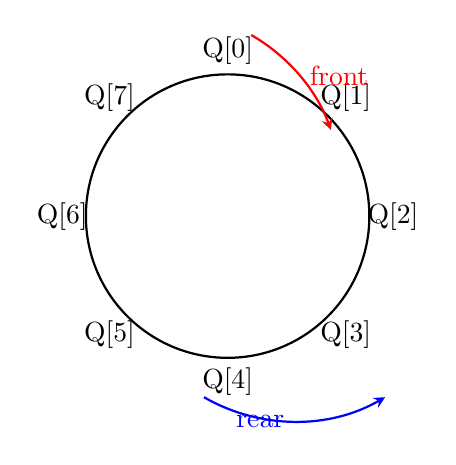
\begin{tikzpicture}[>=stealth, scale=1.0]
% 画一个环形示意
\draw[thick] (0,0) circle (1.8);
\node at (0,2.1) {Q[0]};
\node at (1.5,1.5) {Q[1]};
\node at (2.1,0) {Q[2]};
\node at (1.5,-1.5) {Q[3]};
\node at (0,-2.1) {Q[4]};
\node at (-1.5,-1.5) {Q[5]};
\node at (-2.1,0) {Q[6]};
\node at (-1.5,1.5) {Q[7]};
\draw[->,red,thick] (0.3,2.3) arc (60:20:2.3) node[midway,right] {front};
\draw[->,blue,thick] (-0.3,-2.3) arc (240:300:2.3) node[midway,left] {rear};
\end{tikzpicture}
\end{center}
\end{mydef}

\begin{formula}{循环队列的存储结构与基本操作}{circular-queue-ops}
\textbf{约定：front 指向队头元素，rear 指向队尾元素的下一个空位。}

\begin{lstlisting}[language=C]
#define MaxSize 100
typedef struct {
    ElemType data[MaxSize];
    int front;   // 队头指针
    int rear;    // 队尾指针（指向队尾下一空位）
} SqQueue;
\end{lstlisting}

\textbf{核心操作：}
\begin{lstlisting}[language=C]
// 初始化
void InitQueue(SqQueue *Q) {
    Q->front = Q->rear = 0;
}

// 入队（循环前进）
bool EnQueue(SqQueue *Q, ElemType e) {
    if ((Q->rear + 1) % MaxSize == Q->front)
        return false;                    // 队满
    Q->data[Q->rear] = e;                // 写入队尾
    Q->rear = (Q->rear + 1) % MaxSize;   // rear 循环+1
    return true;
}

// 出队
bool DeQueue(SqQueue *Q, ElemType *e) {
    if (Q->front == Q->rear)
        return false;                    // 队空
    *e = Q->data[Q->front];
    Q->front = (Q->front + 1) % MaxSize; // front 循环+1
    return true;
}

// 队列长度
int QueueLength(SqQueue Q) {
    return (Q.rear - Q.front + MaxSize) % MaxSize;
}
\end{lstlisting}
\end{formula}

\begin{conclusion}{循环队列判空/判满的三种方式}{queue-empty-full}
在上述 \texttt{front} 指向队头、\texttt{rear} 指向队尾下一空位的约定下，\texttt{front == rear} 既是空队条件，也是满队条件——需要额外手段区分：

\begin{tablebox}{判空/判满的三种策略}
\centering
\begin{tabular}{|c|c|c|}
\hline
策略 & 判空 & 判满 \\
\hline
\textbf{① 牺牲一个单元} & \texttt{front == rear} & \texttt{(rear+1)\%MaxSize == front} \\
\textbf{② 增设长度计数} & \texttt{len == 0} & \texttt{len == MaxSize} \\
\textbf{③ 增设 tag 标记} & \texttt{front==rear \&\& tag==0} & \texttt{front==rear \&\& tag==1} \\
\hline
\end{tabular}
\end{tablebox}

策略①是 408 最常用写法，代价是数组有效容量为 $\text{MaxSize}-1$。策略②和③可以充分利用所有单元，但需要额外维护计数器或标记位。tag 标记在每次入队操作时置 1，出队操作时置 0。

\textbf{注意：} 若定义 \texttt{rear} 指向队尾元素（而非下一空位），则需相应调整初始值、入队/出队的顺序和判空/判满条件——408 选择题务必仔细审题。
\end{conclusion}

\subsection{链队列（Linked Queue）}

\begin{mydef}{链队列}{linked-queue}
用链表实现的队列。需要两个指针：\texttt{front} 指向队头结点，\texttt{rear} 指向队尾结点。入队操作在链尾进行，出队操作在链头进行。

通常\textbf{带头结点}：头结点便于统一空队和非空队的操作代码。空队时 \texttt{front == rear}（都指向头结点）。
\end{mydef}

\begin{formula}{链队列的实现}{linked-queue-ops}
\begin{lstlisting}[language=C]
typedef struct QNode {
    ElemType data;
    struct QNode *next;
} QNode;
typedef struct {
    QNode *front;   // 队头指针
    QNode *rear;    // 队尾指针
} LinkQueue;

// 初始化（带头结点）
void InitQueue(LinkQueue *Q) {
    Q->front = Q->rear = (QNode*)malloc(sizeof(QNode));
    Q->front->next = NULL;
}

// 判空
bool QueueEmpty(LinkQueue Q) {
    return Q.front == Q.rear;
}

// 入队（尾插法）
bool EnQueue(LinkQueue *Q, ElemType e) {
    QNode *p = (QNode*)malloc(sizeof(QNode));
    if (!p) return false;
    p->data = e;
    p->next = NULL;
    Q->rear->next = p;   // 原队尾 → 新结点
    Q->rear = p;         // 更新队尾指针
    return true;
}

// 出队
bool DeQueue(LinkQueue *Q, ElemType *e) {
    if (Q->front == Q->rear) return false;   // 队空
    QNode *p = Q->front->next;               // p 指向队头结点
    *e = p->data;
    Q->front->next = p->next;                // 头结点跳过队头
    if (Q->rear == p)                        // 若删除的是最后一个结点
        Q->rear = Q->front;                  // 则 rear 也回到头结点
    free(p);
    return true;
}
\end{lstlisting}

\textbf{注意出队时的特判：} 当队列只剩一个元素时，删除后队尾指针 \texttt{rear} 必须回指头结点，否则 \texttt{rear} 将指向已释放的内存（\textbf{悬挂指针}）。这是 408 常考的细节。
\end{formula}

\subsection{双端队列（Deque）}

\begin{mydef}{双端队列}{deque}
双端队列（Double-Ended Queue, Deque）是允许在\textbf{两端}都进行插入和删除操作的线性表。

根据受限方式分为两类：
\begin{itemize}
    \item \textbf{无限制双端队列}：两端均可入队、出队。
    \item \textbf{输出受限的双端队列}：一端可插入/删除，另一端只能插入。
    \item \textbf{输入受限的双端队列}：一端可插入/删除，另一端只能删除。
\end{itemize}

双端队列是栈和队列的推广：若限定一端只入不出、另一端只出不入，则退化为队列；若限定所有操作在同一端，则退化为栈。
\end{mydef}

\begin{attention}
408 对双端队列的考察通常为选择题：给定输入序列（如 $1,2,3,4$），判断某种双端队列能产生/不能产生哪种输出序列。解题关键——在纸上模拟两端操作的可能性，标记出受限端的操作能力。
\end{attention}

\subsection{栈的应用}

\subsubsection{括号匹配}

\begin{conclusion}{括号匹配算法}{bracket-matching}
检查表达式中的括号（\texttt{()、[]、\{\}}）是否正确配对：
\begin{enumerate}
    \item 扫描表达式，遇\textbf{左括号}则入栈；
    \item 遇\textbf{右括号}：
    \begin{itemize}
        \item 若栈空，则不匹配（右括号多了）；
        \item 弹出栈顶左括号，检查是否与当前右括号同类——不匹配则报错；
    \end{itemize}
    \item 扫描完后，若栈\textbf{非空}则不匹配（左括号多了）；栈空则匹配成功。
\end{enumerate}

\begin{lstlisting}[language=C]
bool BracketMatch(char *expr) {
    SqStack S; InitStack(&S);
    for (int i = 0; expr[i] != '\0'; i++) {
        if (expr[i]=='(' || expr[i]=='[' || expr[i]=='{')
            Push(&S, expr[i]);
        else if (expr[i]==')' || expr[i]==']' || expr[i]=='}') {
            if (StackEmpty(S)) return false;
            char top; Pop(&S, &top);
            if ((expr[i]==')' && top!='(') ||
                (expr[i]==']' && top!='[') ||
                (expr[i]=='}' && top!='{'))
                return false;
        }
    }
    return StackEmpty(S);  // 最后栈空才匹配
}
\end{lstlisting}
时间复杂度 $O(n)$，空间复杂度 $O(n)$。
\end{conclusion}

\subsubsection{表达式求值}

\begin{mydef}{中缀、后缀与前缀表达式}{expression-notation}
\begin{itemize}
    \item \textbf{中缀表达式}（Infix）：运算符在两个操作数之间。如 $A+B$。符合人类习惯，但需要括号和优先级规则。
    \item \textbf{后缀表达式}（Postfix / 逆波兰表示法）：运算符在操作数之后。如 $AB+$。无需括号，天然适合栈计算。
    \item \textbf{前缀表达式}（Prefix / 波兰表示法）：运算符在操作数之前。如 $+AB$。
\end{itemize}
408 重点考察\textbf{中缀转后缀}的过程和\textbf{后缀表达式求值}。
\end{mydef}

\begin{conclusion}{中缀表达式转后缀表达式}{infix-to-postfix}
\textbf{算法（算符优先法）：}
\begin{enumerate}
    \item 初始化一个\textbf{运算符栈}（存运算符和左括号），结果队列存后缀表达式；
    \item 从左到右扫描中缀表达式的每个 token：
    \begin{itemize}
        \item \textbf{操作数}：直接输出（进入后缀表达式）；
        \item \textbf{左括号 \texttt{(}}：入栈；
        \item \textbf{右括号 \texttt{)}}：依次弹出栈顶运算符并输出，直到遇到左括号（左括号出栈但不输出）；
        \item \textbf{运算符}：若其优先级\textbf{高于}栈顶，则入栈；否则，反复弹出栈顶优先级\textbf{不低于}当前运算符的运算符并输出，然后将当前运算符入栈。
    \end{itemize}
    \item 扫描完毕后，将栈中剩余运算符依次弹出输出。
\end{enumerate}

\textbf{运算符优先级（408 标准，不含函数、位运算）：}
\begin{tablebox}{运算符优先级表（优先级数字越大越高）}
\centering
\begin{tabular}{|c|c|c|}
\hline
运算符 & 优先级 & 结合性 \\
\hline
\texttt{*}~~~\texttt{/~~\%} & 3 & 左结合 \\
\texttt{+}~~~\texttt{-} & 2 & 左结合 \\
\texttt{(} & 1（入栈后视为最低）& — \\
\hline
\end{tabular}
\end{tablebox}

\begin{examplebox}
\textbf{示例：} $A+B*(C-D)-E/F$ 转后缀：
\begin{center}
\begin{tabular}{|c|c|c|}
\hline
当前 token & 栈（栈底→栈顶）& 输出 \\
\hline
A & 空 & A \\
+ & + & A \\
B & + & AB \\
* & + * & AB \\
( & + * ( & AB \\
C & + * ( & ABC \\
- & + * ( - & ABC \\
D & + * ( - & ABCD \\
) & + * & ABCD- \\
- & - & ABCD-*+ \\
E & - & ABCD-*+E \\
/ & - / & ABCD-*+E \\
F & - / & ABCD-*+EF \\
结束 & 空 & ABCD-*+EF/ \\
\hline
\end{tabular}
\end{center}
结果为 $ABCD-*+EF/$。
\end{examplebox}
\end{conclusion}

\begin{conclusion}{后缀表达式求值}{postfix-evaluate}
\textbf{算法：}
\begin{enumerate}
    \item 初始化一个\textbf{操作数栈}；
    \item 从左到右扫描后缀表达式；
    \begin{itemize}
        \item \textbf{操作数}：入栈；
        \item \textbf{运算符}：弹出栈顶两个操作数（先弹出的是右操作数，后弹出的是左操作数），计算后结果入栈。
    \end{itemize}
    \item 最终栈中唯一元素即表达式的值。
\end{enumerate}

\begin{lstlisting}[language=C]
// 计算后缀表达式（操作数为整数，运算符 + - * /）
int EvalPostfix(char *postfix) {
    SqStack S; InitStack(&S);
    for (int i = 0; postfix[i]; i++) {
        if (isdigit(postfix[i])) {
            Push(&S, postfix[i] - '0');       // 操作数入栈
        } else {                              // 运算符
            int b, a; Pop(&S, &b); Pop(&S, &a); // b 先弹出（右操作数）
            switch (postfix[i]) {
                case '+': Push(&S, a + b); break;
                case '-': Push(&S, a - b); break;
                case '*': Push(&S, a * b); break;
                case '/': Push(&S, a / b); break;
            }
        }
    }
    int result; Pop(&S, &result);
    return result;
}
\end{lstlisting}
\end{conclusion}

\begin{attention}
\textbf{408 中缀转后缀易错点：}
\begin{enumerate}
    \item 左括号入栈后\textbf{优先级最低}——只有右括号才能让它出栈；
    \item 相同优先级运算符，左结合时，栈内优先级\textbf{高于}栈外优先级（即先算左边的），所以当前运算符\textbf{不高于}栈顶时就要弹出栈顶；
    \item 后缀表达式中操作数的顺序与中缀表达式\textbf{完全相同}——只有运算符位置改变。
\end{enumerate}
\end{attention}

\subsubsection{递归与栈}

\begin{conclusion}{递归的工作栈}{recursion-stack}
递归函数的调用过程天然符合栈的 LIFO 特性。每次函数调用时，系统将返回地址、局部变量、参数等信息压入\textbf{调用栈}（Call Stack），返回时弹出。

以阶乘为例：
\begin{lstlisting}[language=C]
int Factorial(int n) {
    if (n == 0 || n == 1) return 1;     // 递归基
    return n * Factorial(n - 1);         // 递归调用
}
// Factorial(4):
// 调用: fact(4) → fact(3) → fact(2) → fact(1)
// 返回: 1 → 2 → 3 → 4 → 24
\end{lstlisting}

递归与栈的关系：
\begin{itemize}
    \item 任何递归算法都可以用栈\textbf{机械地}转换为非递归算法；
    \item 递归函数本质是通过系统栈保存状态，自己显式维护栈可以达到同样的效果；
    \item 递归到非递归的转换有时能避免系统栈溢出（如用迭代 + 显式栈模拟深度优先遍历）。
\end{itemize}

408 常考点：给定一段递归代码，要求模拟调用栈的变化过程，或分析递归深度（即栈的最大深度）。
\end{conclusion}

\subsection{队列的应用}

\begin{conclusion}{层次遍历（BFS）}{level-order}
队列是实现\textbf{广度优先遍历}（BFS, Breadth-First Search）的核心数据结构。

以二叉树的层次遍历为例（详细见第 4 章）：
\begin{enumerate}
    \item 根结点入队；
    \item 当队列非空时：出队一个结点并访问之；将其左、右孩子（若存在）依次入队；
    \item 重复步骤 2 直到队列为空。
\end{enumerate}

\begin{lstlisting}[language=C]
// 二叉树层次遍历（假设已定义 BiTree 类型）
void LevelOrder(BiTree T) {
    SqQueue Q; InitQueue(&Q);
    if (T) EnQueue(&Q, T);
    while (!QueueEmpty(Q)) {
        BiTree p; DeQueue(&Q, &p);
        visit(p);                        // 访问结点
        if (p->lchild) EnQueue(&Q, p->lchild);
        if (p->rchild) EnQueue(&Q, p->rchild);
    }
}
\end{lstlisting}

队列保证同一层的结点按从左到右的顺序被访问——这是 BFS 的关键性质。
\end{conclusion}

\begin{conclusion}{缓冲区与生产者-消费者}{buffer-queue}
在操作系统中，队列广泛用于\textbf{缓冲区}管理：
\begin{itemize}
    \item \textbf{打印机缓冲队列}：多个打印任务按提交顺序排队等待打印；
    \item \textbf{消息队列}：生产者将消息入队，消费者从队头取出处理；
    \item \textbf{CPU 就绪队列}：就绪进程按优先级/时间片排队等待调度。
\end{itemize}

队列的 FIFO 特性天然保证了处理顺序的公平性。
\end{conclusion}

\subsection{栈与队列的 408 高频考点}

\begin{conclusion}{408 选择/填空常考公式与结论}{stack-queue-keypoints}
\begin{enumerate}
    \item \textbf{循环队列的指针与元素个数}：
    \[
    \text{元素个数} = (\text{rear} - \text{front} + \text{MaxSize}) \bmod \text{MaxSize}
    \]
    其中 \texttt{front} 指向队头，\texttt{rear} 指向队尾下一空位。

    \item \textbf{循环队列判满}（牺牲一单元时）：
    \[
    (\text{rear} + 1) \bmod \text{MaxSize} = \text{front}
    \]

    \item \textbf{共享栈判满}：
    \[
    \text{top1} + 1 = \text{top2}
    \]

    \item \textbf{$n$ 个元素入栈，可能的出栈序列数}（Catalan 数）：
    \[
    C_n = \frac{1}{n+1}\binom{2n}{n}
    \]
    例如 $n=3$ 时，共有 $C_3 = 5$ 种可能的出栈序列（全排列 $3! = 6$ 种中，$3,1,2$ 不可能合法出栈）。

    \item \textbf{合法出栈序列的判断}：对任意三个元素 $i<j<k$，若 $k$ 先于 $i$ 和 $j$ 出栈，则 $i$ 必须后于 $j$ 出栈（大元素先出，则其后的小元素出栈顺序必须与入栈顺序相反）。

    \item \textbf{中缀转后缀的手工方法}：
    \begin{itemize}
        \item 将所有运算用括号显式标注优先级（全括号化）；
        \item 将运算符移到对应右括号之后；
        \item 去掉所有括号。
    \end{itemize}
    例如 $A+B*C \to (A+(B*C)) \to A\ B\ C\ *\ +$。

    \item \textbf{后缀表达式求值}：弹出时第一个是右操作数，第二个是左操作数——减法和除法不可交换顺序。
\end{enumerate}
\end{conclusion}

\begin{attention}
\textbf{408 真题反复考察的循环队列细节：}
\begin{enumerate}
    \item 题目可能使用不同的指针定义（front 指向队头前一位置、rear 指向队尾元素等），判空/判满条件和入队/出队操作步骤必须根据题设推导，切忌死记硬背公式。
    \item 已知 front 和 rear 的值求元素个数时，使用模运算公式，注意 MaxSize 的具体值。
    \item 「最多能存储多少个元素」——若采用牺牲一单元的方式，答案为 $\text{MaxSize}-1$；否则为 $\text{MaxSize}$。
\end{enumerate}
\end{attention}

\newpage
\section{习题}

\subsection{基础过关题}

\begin{enumerate}

\item \textbf{（2009年·单选·2）} 设栈S的初始状态为空，入栈序列为$1,2,3,\ldots,n$，若出栈序列的第一个元素是$k$（$1\leqslant k\leqslant n$），则以下说法正确的是
\begin{center}
\begin{tabular}{ll}
(A) 此时元素$1,2,\ldots,k-1$必定全部在栈中，且$1$在栈底 \\
(B) 第$i$个出栈元素必定是$n-i+1$ \\
(C) 出栈序列的个数与$k$无关 \\
(D) 出栈序列的可能个数为$C_{n-1}^{k-1}$
\end{tabular}
\end{center}

\item \textbf{（2010年·单选·1）} 设循环队列的存储空间为$Q[0..m-1]$，\texttt{front}指向队头元素，\texttt{rear}指向队尾元素的下一位置。则元素入队时\texttt{rear}的变化为
\begin{center}
\begin{tabular}{ll}
(A) \texttt{rear = rear + 1} & (B) \texttt{rear = (rear + 1) \% (m - 1)} \\[6pt]
(C) \texttt{rear = (rear + 1) \% m} & (D) \texttt{rear = (rear + 1) \% (m + 1)}
\end{tabular}
\end{center}

\item \textbf{（2012年·单选·2）} 中缀表达式$A+B*(C-D)-E/F$对应的后缀表达式是
\begin{center}
\begin{tabular}{ll}
(A) $ABCD-*+EF/-$ & (B) $AB+CD-*EF/-$ \\[6pt]
(C) $ABCD-*+EF/$ & (D) $AB+CD-*E-F/$
\end{tabular}
\end{center}

\item \textbf{（2023年·单选·1）} 对后缀表达式$ab+c*d-ef+/$进行求值（设$a,b,c,d,e,f$均为操作数），在从左到右扫描求值的过程中，操作数栈中元素个数的最大值为
\begin{center}
\begin{tabular}{ll}
(A) 2 & (B) 3 \\[6pt]
(C) 4 & (D) 5
\end{tabular}
\end{center}

\item \textbf{（2018年·单选·2）} 设用数组$A[0..n-1]$实现两个栈共享存储空间的共享栈。栈1的栈底在$A[0]$处，从低地址向高地址增长；栈2的栈底在$A[n-1]$处，从高地址向低地址增长。\texttt{top1}指向栈1的栈顶元素，\texttt{top2}指向栈2的栈顶元素。则栈满的条件是
\begin{center}
\begin{tabular}{ll}
(A) $\texttt{top1} + \texttt{top2} = n$ & (B) $\texttt{top1} + 1 = \texttt{top2}$ \\[6pt]
(C) $\texttt{top1} = \texttt{top2}$ & (D) $\texttt{top1} + 1 < \texttt{top2}$
\end{tabular}
\end{center}

\item \textbf{（2014年·单选·1）} 设循环队列的存储空间为$Q[0..m-1]$，\texttt{front}指向队头元素，\texttt{rear}指向队尾元素的下一位置。在采用「牺牲一个存储单元」判满策略时，队列为空的判定条件是
\begin{center}
\begin{tabular}{ll}
(A) $\texttt{front} = \texttt{rear}$ & (B) $(\texttt{rear}+1) \bmod m = \texttt{front}$ \\[6pt]
(C) $\texttt{front} = 0$ 且 $\texttt{rear} = 0$ & (D) $\texttt{front} = (\texttt{rear}+1) \bmod m$
\end{tabular}
\end{center}

\end{enumerate}

\subsection{综合训练}

\begin{enumerate}[resume]

\item \textbf{（2019年·单选·3）} 以下算法中，需要使用队列作为辅助数据结构的是
\begin{center}
\begin{tabular}{ll}
(A) 二叉树的先序遍历 & (B) 二叉树的层次遍历 \\[6pt]
(C) 图的深度优先遍历 & (D) 中缀表达式转后缀表达式
\end{tabular}
\end{center}

\item \textbf{（综合题）} 给定入栈序列$\{1,2,3,4,5\}$，请：
\begin{enumerate}
    \item[(1)] 列出所有以3开头、以5结尾的合法出栈序列；
    \item[(2)] 说明推导过程与判断合法性的关键原则。
\end{enumerate}

\item \textbf{（综合题）} 设循环队列$Q[0..M-1]$，\texttt{front}指向队头元素，\texttt{rear}指向队尾元素的下一个空位。回答以下问题：
\begin{enumerate}
    \item[(1)] 写出队列中元素个数的计算公式；
    \item[(2)] 若$M=10$，$\texttt{front}=6$，$\texttt{rear}=3$，求队列中元素个数；
    \item[(3)] 若采用「牺牲一个单元」策略，分别写出判空和判满条件。
\end{enumerate}

\end{enumerate}

\vspace{8pt}
\noindent\textbf{拓展阅读：}
\begin{itemize}
    \item 邓俊辉《数据结构（C++语言版）》第4章「栈与队列」——表达式求值的完整实现。
    \item Sedgewick《算法》第1.3节——栈与队列的ADT定义与迭代器设计。
\end{itemize}
